Before Transformer (see Section \ref{section:transformer}), U-Net \cite{ronneberger2015u} was popular for semantic segmentation task. Segmentation Transformer (SETR) \cite{zheng2021rethinking} was one of early applications of Transformer for semantic segmentation, achieving considerable improvement over CNNs. SegFormer \cite{xie2021segformer} was developed in motivation of this work, with Efficient Self-attention. Recently, Segment Anything Model (SAM) \cite{kirillov2023segment} was designed for the ability to run on low-end devices. In this section, we discuss two latest models, SegFormer and SAM, which are also those used in our watermark segmentation phase.

\subsection{SegFormer}
\label{intro:segformer}
SegFormer made use of multi-head attention mechanism, but highly specialized for semantic segmentation task.

\begin{figure}[ht]
  \centering
  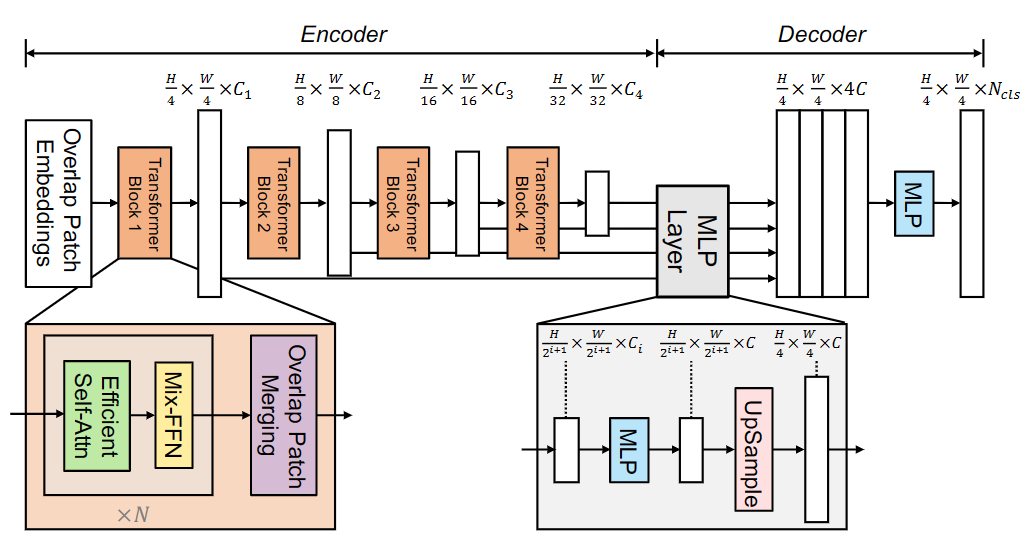
\includegraphics[width=0.7\linewidth]{img/segformer.png}
  \vspace{0.5cm}
  \caption{SegFormer Architecture}
  \label{figure:segFormer-architecture}
\end{figure}

As can be seen in Figure \ref{figure:segFormer-architecture}, there are two major components in the architecture, namely the Overlap Patch Embedding, Transformer Block and the MLP Layer, whose details are delved into in following sections.

\subsubsection{Encoder}

\textbf{Overlap Patch Embedding.} Originally in Vision Transformer (ViT) \cite{dosovitskiy2020image}, an image of size $H\times W\times 3$ is divided into $\frac{HW}{P^2}$ patches of size $P\times P \times 3$. Each patch is then flattened and linearly projected in to a $C$-dimensional vector, where $C>3$, returning a sequence of size $\frac{HW}{P^2}\times C$. The patches in this case have no overlaps.

SegFormer employed Overlap Patch Embedding, with two additional hyperparameters $s$ and $p$ for stride and padding, similarly to CNNs. In particular, the authors of SegFormer used $(P,s,p)\in\{(7,4,3), (3,2,1)\}$, result in a sequence size $\frac{HW}{4} \times C$, while preserved the local continuity around those patches.

\textbf{Efficient Self-Attention.} This is an subblock of the Transformer block. After extracted as the keys $\mathbf{K}$ and queries $\mathbf{Q}$ of the same size as the sequence, the matrices go through a self-reduction process of ratio $r$. For instance, let $N=\frac{HW}{4}$, we have
\begin{align*}
  \mathbf{K'} & = \mathrm{Reshape}\left(\dfrac{N}{r}, C\cdot r\right)(\mathbf{K}) \\
  \mathbf{K}  & = \mathrm{Linear}\left(\dfrac{N}{r}, C\right)(\mathbf{K'}).
\end{align*}
Thus, $\mathbf{K}$ is reduced to dimension $\frac{N}{r}\times C$ and similarly for $\mathbf{Q}$. The complexity is reduced from $O(N^2)$ to $O\left(\frac{N^2}{r}\right)$ comparing to original Multi-head Attention \cite{xie2021segformer}. In particular, the matrices $\mathbf{K}$, $\mathbf{Q}$ and $\mathbf{V}$ are constrained to be of equal size, enabling them to be generated simultaneously from the token sequence, which results in improved computational performance.

\textbf{Mix-FFN.} This subblock is used as an alternative to Positional Encoding in ViT that only takes care of the distance between the tokens. The approach in ViT leads to the drop of accuracy for semantic segmentation task when the test set resolution differs from the training set. In SegFormer, the authors included a convolutional layer to encode positional information
$$\xbf_{\mathrm{out}} = \mathrm{MLP}(\mathrm{GELU}(\mathrm{Conv_{3\times 3}(\mathrm{MLP}(\xbf_{in}))})).$$
Their approach was based on an argument that adding PE to feature map is not necessary in semantic segmentation, and was empirically proved to be sufficient for this task.


\textbf{Overlapped Patch Merging.} This is the final subblock of the Transformer block that reshapes the previous output to size $\frac{W}{2}\times \frac{H}{2} \times C$, and processes similarly to Overlap Patch Embedding, returning a sequence of size $\frac{WR}{16}\times C_1$, where $C_1>C$. The other three following Transformer Blocks work similar, getting the sequence after the previous block and outputting a sequence of size $\frac{WR}{2^{2i+2}}\times C_i$, for $i\in\{2,3,4\}$.

\subsubsection{Decoder}
After each Transformer Block, the sequence is reshaped to get hierarchical representation of size $\frac{W}{2^{i+1}}\times \frac{H}{2^{i+1}}\times C_i$, for $i\in{1,2,3,4}$. Each representation goes through an MLP and then is unsampled to size $\frac{W}{4}\times \frac{H}{4}\times 3$. The representations are concatenated to $\frac{W}{4}\times \frac{H}{4}\times 12$. The last MLP (the blue block in Figure \ref{figure:segFormer-architecture}) gives the output $\frac{W}{4}\times \frac{H}{4}\times N_{\mathrm{cls}}$, where $N_{\mathrm{cls}}$ is the number of classes. Intersection over Union (mIoU) was selected to be the loss function.

\subsection{Segment Anything}
\label{sec:intro-sam}
The other choice for the watermark detection stage in our pipeline is the Segment Anything model (SAM) developed by Meta \cite{kirillov2023segment}, a considerable revolution in semantic segmentation task, as it allows prompts from user. The design is claimed to be optimized to work in real-time. The model consists of an image encoder, a prompt encoder and a lightweight mask decoder. We will delve into the details as follows.

\begin{figure}
  \centering
  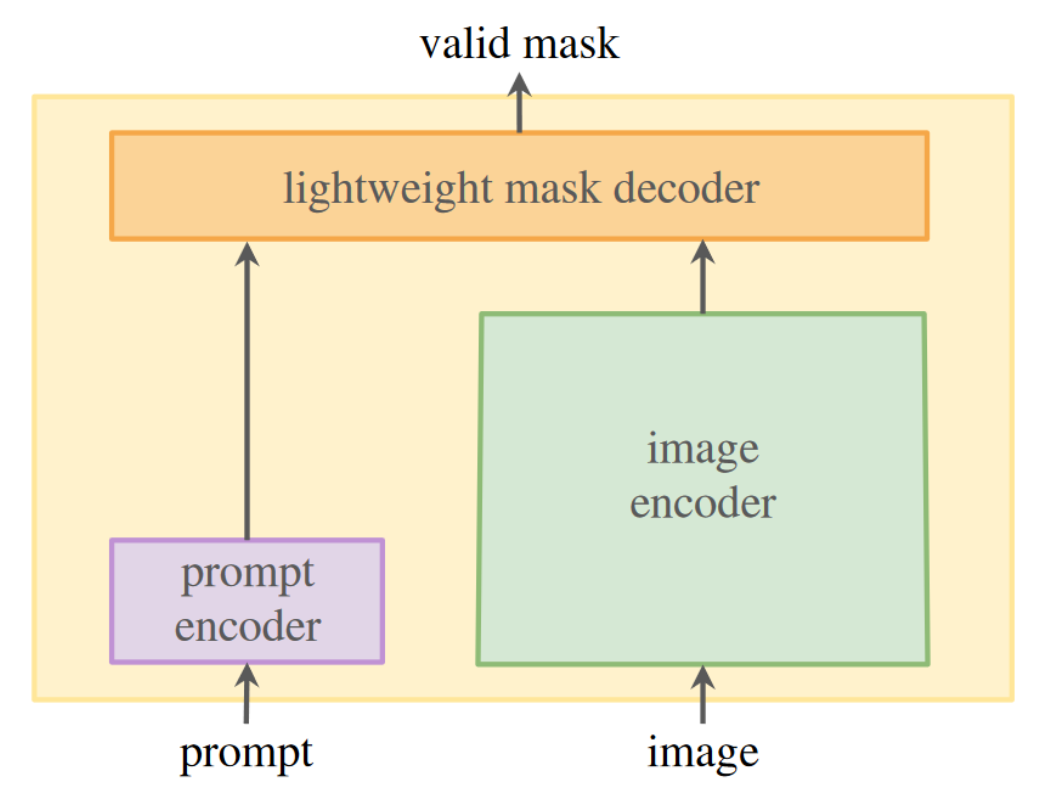
\includegraphics[width=0.6\textwidth]{img/segment-anything-model.png}
  \vspace{0.25cm}
  \caption[The overall architecture of Segment Anything model]{The overall architecture of Segment Anything model \cite{kirillov2023segment}}
\end{figure}

\subsubsection{Image Encoder}
The authors of the Segment Anything model followed standard practices, that they firstly rescale an image and pad the shorter side to attain an input resolution of $1024\times1024$. They employed several ViT backbones \cite{dosovitskiy2020image}, one of them is a ViT-H/16, followed by a Masked Autoencoder \cite{he2022masked}, returning an image of 16-time lower resolution. The image is then passed through convolutional layers to arrive at an output size of $256\times 64\times 64$.

\subsubsection{Prompt Encoder}
The model allows prompts of two types: sparse (points, boxes, text) and dense (masks). Each prompt is mapped to a $256$-dimensional vectorial embedding. A point is represented by the sum of a foreground-background learned embedding and a positional encoding. The latter value is a general approach of the sinusoid function called Fourier features \cite{tancik2020fourier}. A box is represented by an representation pair. For the top-left corner, the representation is the sum its positional encoding and its learned ``top-left corner'' embedding. A similar structure is applied for the bottom-right corner, except for that a learned ``bottom-right corner'' embedder is used. A text encoder can be any available one. The authors used continuous bag of words and Text Transformer \cite{vaswani2017attention} for their experiments. A mask is firstly converted a 4-time lower resolution than the input image. Then it is downscaled  by additional 4 times, using two $\mathrm{Conv}_{2\times 2}$ with stride 2 and output channels 4 and 16, respectively. A final $\mathrm{Conv}_{1\times 1}$ maps the channel dimension to $256$. Each layer is separated by GELU activations and layer normalization. Finally, the mask are added to the image element-wise. If there is no mask prompt, a learned embedding representing ``no mask'' is added to each image embedding location.

\subsubsection{Lightweight Mask Decoder}
The previous image embedding is treated as a set of $64^2$ 256-dimensional vectors. The lightweight mask decoder is designed using Cross Attention (see Section \ref{section:transformer}), as illustrated in Figure \ref{figure:segment-anything-model-mask-decoder}.

\begin{figure}[ht]
  \centering
  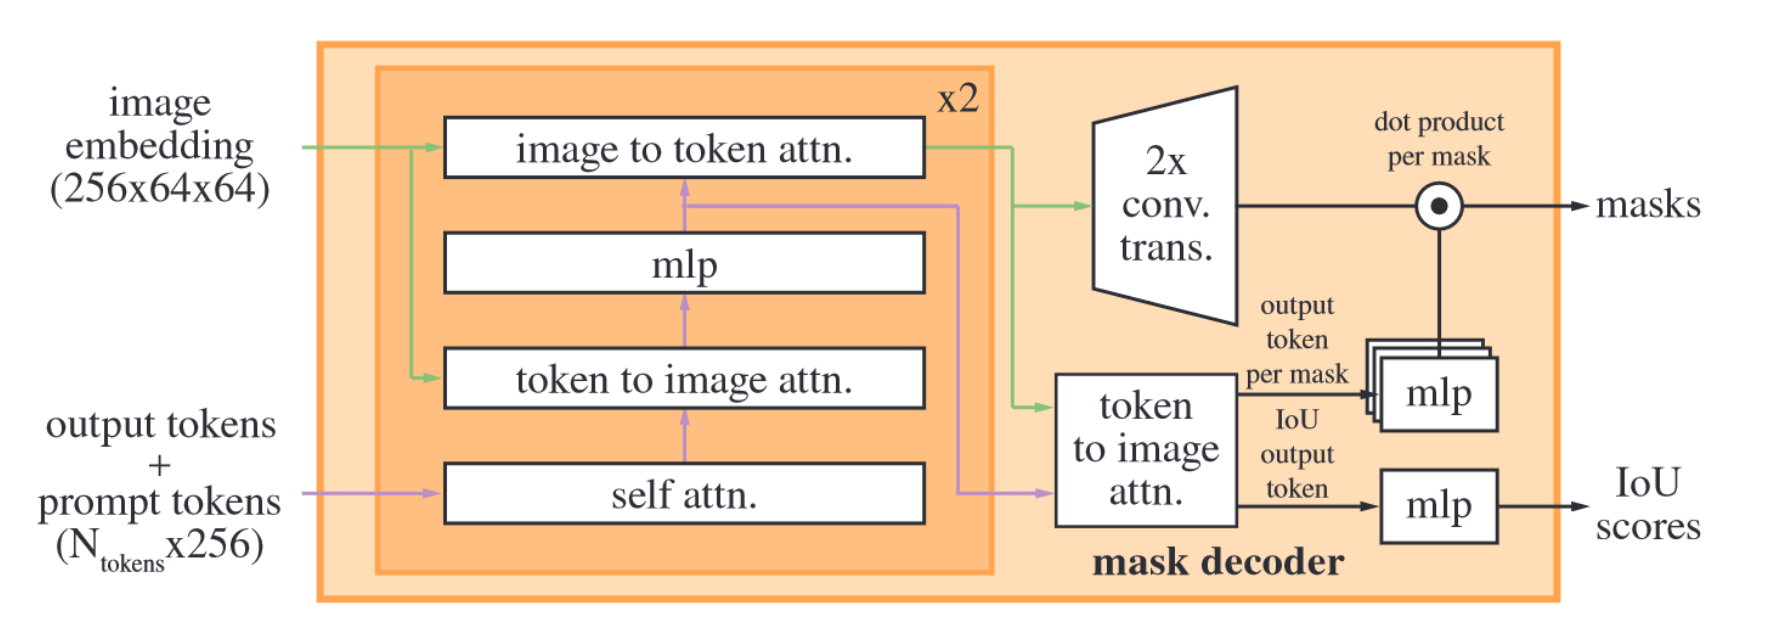
\includegraphics[width=0.6\textwidth]{img/segment-anything-model-mask-decoder.png}
  \vspace{0.25cm}
  \caption[The lightweight mask decoder design]{The lightweight mask decoder design \cite{kirillov2023segment}}
  \label{figure:segment-anything-model-mask-decoder}
\end{figure}

\begin{figure}[H]
  \centering
  \begin{subfigure}[b]{0.48\textwidth}
    \centering
    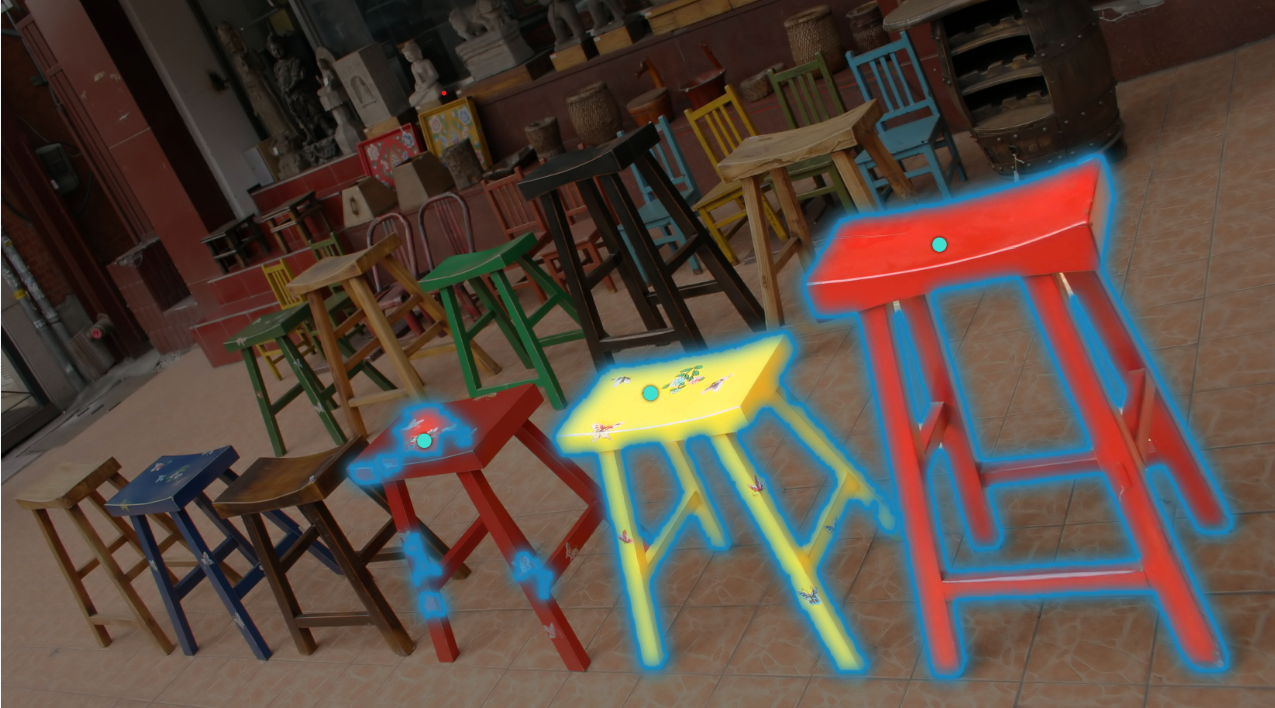
\includegraphics[width=\textwidth]{img/sam-segmented-after-point.png}
    \label{fig:sam_point}
  \end{subfigure}
  \hfill
  \begin{subfigure}[b]{0.48\textwidth}
    \centering
    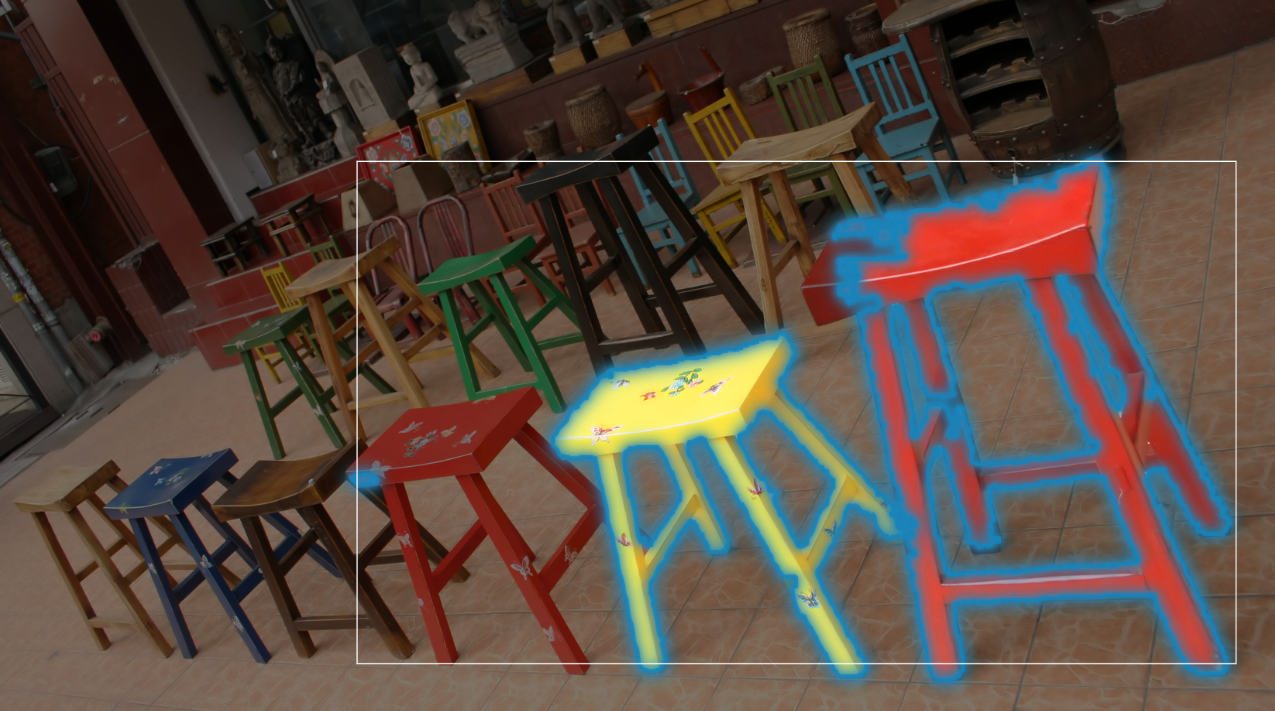
\includegraphics[width=\textwidth]{img/sam-segment-bounding-box.png}
    \label{fig:sam_box}
  \end{subfigure}
  \caption[Segmented regions returned by SAM]{Segmented regions returned by SAM. In the left figure, three points are selected, while in the right figure, a box is drawn. In both cases, the leftmost chair is not fully recognized.}
  \label{fig:sam_segments}
\end{figure}
